%%%%%%%%%%%%%%%%%%%%%%%%%%%%%%%%%%%%%%%%%%%%%%%%%%%%%%%%%%%%%%%%%%%%%%%%%%%
%
% Plantilla para un artículo en LaTeX en español.
%
%%%%%%%%%%%%%%%%%%%%%%%%%%%%%%%%%%%%%%%%%%%%%%%%%%%%%%%%%%%%%%%%%%%%%%%%%%%

% Qué tipo de documento estamos por comenzar:
\documentclass[a4paper]{article}
% Esto es para que el LaTeX sepa que el texto está en español:
\usepackage[spanish]{babel}
\selectlanguage{spanish}
% Esto es para poder escribir acentos directamente:
\usepackage[utf8]{inputenc}
\usepackage[T1]{fontenc}
\usepackage{float}

\usepackage{enumerate} 

%% Asigna un tamaño a la hoja y los márgenes
\usepackage[a4paper,top=3cm,bottom=2cm,left=3cm,right=3cm,marginparwidth=1.75cm]{geometry}

%% Paquetes de la AMS
\usepackage{amsmath, amsthm, amsfonts}
%% Para añadir archivos con extensión pdf, jpg, png or tif
\usepackage{graphicx}
\usepackage[colorinlistoftodos]{todonotes}
\usepackage[colorlinks=true, allcolors=blue]{hyperref}

%% Primero escribimos el título
\title{Analisis de algoritmos de ordenamiento }
\author{Bejar Merma Ángel Andrés\\
  \small Universidad Nacional de San Agustin\\
  \small andresbjar97@gmail.com\\
  \small Ciudad de Arequipa
  \date{}
}

%% Después del "preámbulo", podemos empezar el documento

\begin{document}
%% Hay que decirle que incluya el título en el documento
\maketitle

%% Aquí podemos añadir un resumen del trabajo (o del artículo en su caso) 
\begin{abstract}
Esta es una plantilla simple para crear un articulo \LaTeX en español, con algunos comandos que se usarán frecuentemente para hacer tareas de la licenciatura en Física.
\end{abstract}

%% Iniciamos "secciones" que servirán como subtítulos
%% Nota que hay otra manera de añadir acentos
\section{Introducci\'on}

¡Tu introducción va aquí! A continuación, se enumeran algunos ejemplos de comandos y funciones de uso común para ayudarte a comenzar.

cuaderno de trabajo\cite{colab}

\begin{enumerate}[a)]
\item
\item
\item


\end{enumerate}



\subsection{Implemente los siguientes algoritmos en tres lenguajes de programación}





\section{Marco Teórico}

\section{Metodología}

\begin{enumerate}[a)]

\item Bubble sort

\item Heap sort

\item Insertion sort

\item Selection sort

\item Shell sort

\item  Merge sort

\item Quick sort
\end{enumerate}


\begin{figure}[H]%primero aqui sino arriba sino abajo
\centering
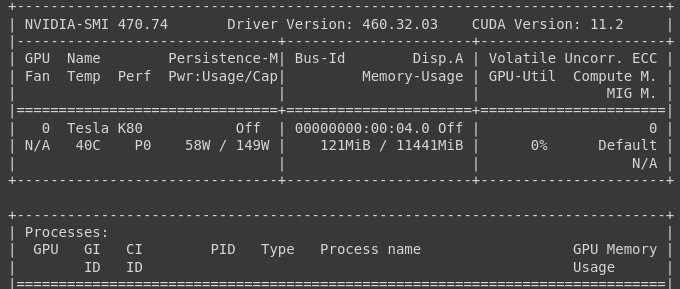
\includegraphics[width=10cm]{imagenes/arq2.png}
\caption{}
\end{figure}

\begin{figure}[H]%primero aqui sino arriba sino abajo
\centering
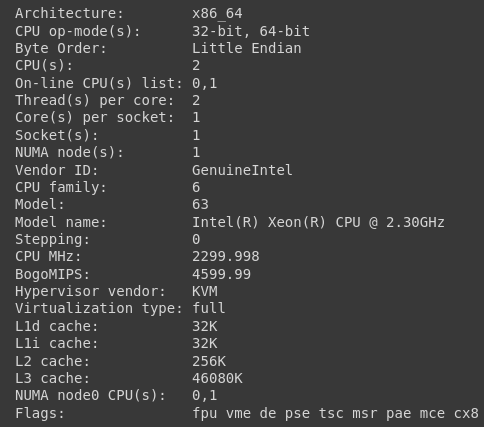
\includegraphics[width=7cm]{imagenes/arquitectura2.png}
\caption{}
\end{figure}


\begin{figure}[H]%primero aqui sino arriba sino abajo
\centering
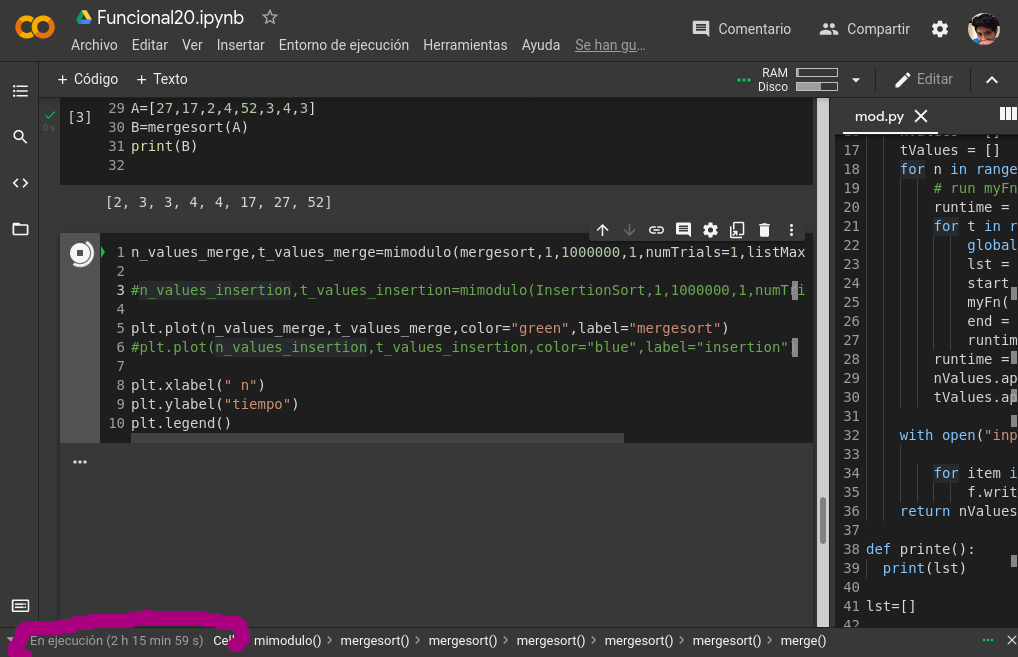
\includegraphics[width=14cm]{imagenes/cap.png}
\caption{}
\end{figure}

\begin{figure}[H]%primero aqui sino arriba sino abajo
\centering
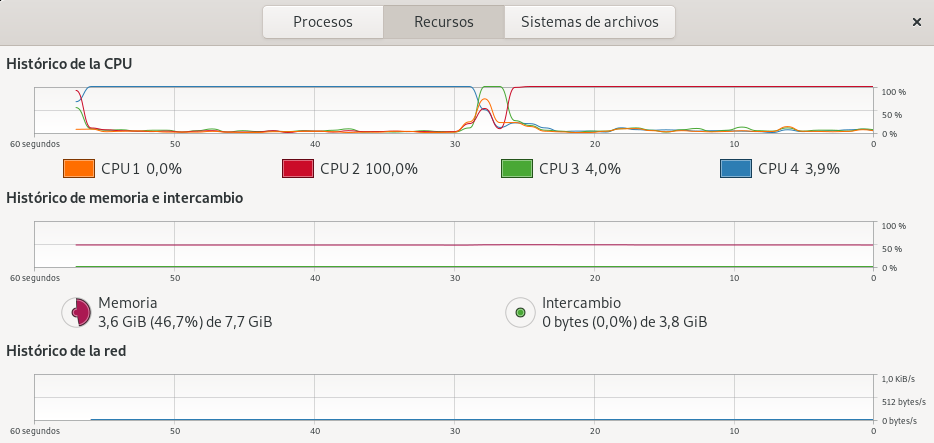
\includegraphics[width=13cm]{imagenes/cpus.png}
\caption{}
\end{figure}



\section{Resultados}

\section{Conclusiones}


\section{Discusión}



Documentar sus hallazgos en un formato de artículo de investigación (formato de libre elección), considerando
aspectos del marco teórico (estado del arte), metodología, resultados, conclusiones, discusión y bibliografía \cite{fager}.

\bibliographystyle{plain}
\bibliography{referencias}




\end{document}
